% 3章
\chapter{数値実験}

研究で新たに実装した歩行者工一ジェントおよび歩車相互作用モデルの定量的な評価性能を検証するために,シミュレーション実験を行った.
この章では、実験で用いた環境設定と、実験結果をどのような評価指標で判断したか、またその結果と考察についてまとめている。

\section{実験条件}

今回の実験では、図\ref{environment}に示すように、15m四方の二次元平面と、排泄場所としてのトイレをその上部に設置した。

\begin{figure}[htb]
\begin{center}
 
\includegraphics[scale=0.6]{figures/environment.png}
 \caption[実験環境]{実験環境 \label{environment}}
\end{center}
\end{figure}

この環境の中で、介護者と被介護者の可視化をおこなっていく。今回の実験では、介護における技術を導入した際に、それが介護環境にどのようなインパクトをあたえるのかについて検証を行うことが目的であるので、介護者の数は1人、被介護者の数は16人と設定し、比較的大きい施設を対象とした。
被介護者のバリエーションとしては、健常者(技術のサポートを受けている被介護者)、頻尿である被介護者、認知症等の要因によってトイレにいくというアラートを出すことが難しい状況にある被介護者の3種類を想定している。
それぞれ図\ref{elderly_v1}、図\ref{elderly_v2}、図\ref{elderly_v3}に示しているように、可視化の際に形を変えることでエージェントがそれぞれどのように相互作用を行っているのかを見ることができる。

\begin{figure}[htb]
\begin{center}
 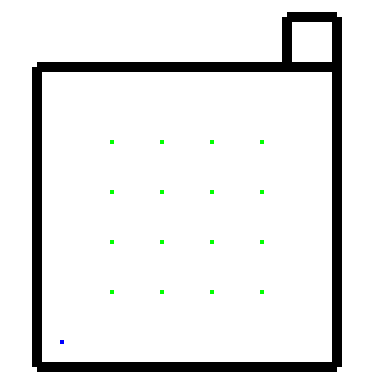
\includegraphics[scale=0.6]{figures/elderly_v1.png}
 \caption[健常者(介護技術を導入した場合の被介護者)の場合の可視化]{健常者(介護技術を導入した場合の被介護者)の場合の可視化 \label{elderly_v1}}
\end{center}
\end{figure}

\begin{figure}[htb]
\begin{center}
 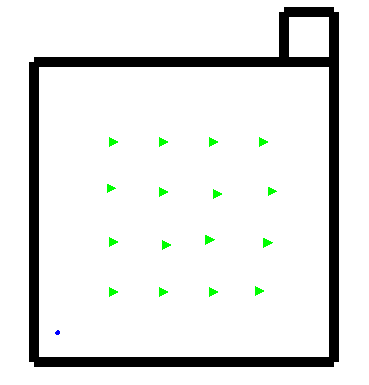
\includegraphics[scale=0.6]{figures/elderly_v2.png}
 \caption[頻尿の場合の可視化]{頻尿の場合の可視化 \label{elderly_v2}}
\end{center}
\end{figure}

\begin{figure}[htb]
\begin{center}
 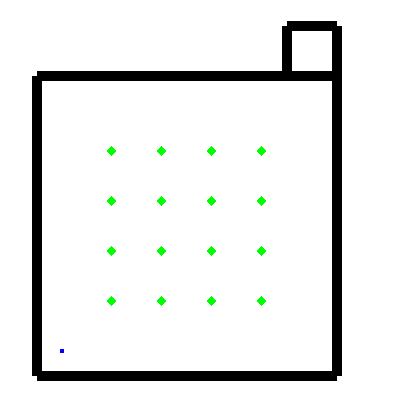
\includegraphics[scale=0.6]{figures/elderly_v3.png}
 \caption[認知症の場合の可視化]{認知症の場合の可視化 \label{elderly_v3}}
\end{center}
\end{figure}

この3種類のエージェントが、介護施設内の自由時間である2時間の間にいかなる回数排泄介助を行うことが必要か、またその介助は本当に必要であったのかということを確かめる実験をおこなう。
一般的に高齢者の排尿量は一回で100-150mlで、1日に8−10回ほどトイレで尿を行うことが知られているので、今回の実験ではそちらの数値を用いることとした。
健常者の場合は、
頻尿の場合は、
認知症の場合は、
この3種類を〜のように組み合わせた6パターンにおいて、相互作用を確認することとする。

\begin{figure}[htb]
\begin{center}
 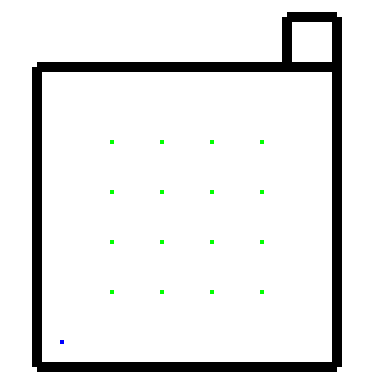
\includegraphics[scale=0.6]{figures/elderly_v1.png}
 \caption[健常者(介護技術を導入した場合の被介護者)の場合の可視化]{健常者(介護技術を導入した場合の被介護者)の場合の可視化 \label{elderly_v1}}
\end{center}
\end{figure}

\begin{figure}[htb]
\begin{center}
 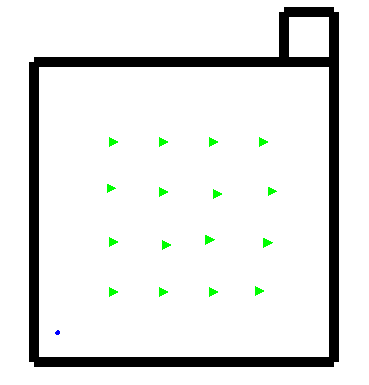
\includegraphics[scale=0.6]{figures/elderly_v2.png}
 \caption[頻尿の場合の可視化]{頻尿の場合の可視化 \label{elderly_v2}}
\end{center}
\end{figure}

\begin{figure}[htb]
\begin{center}
 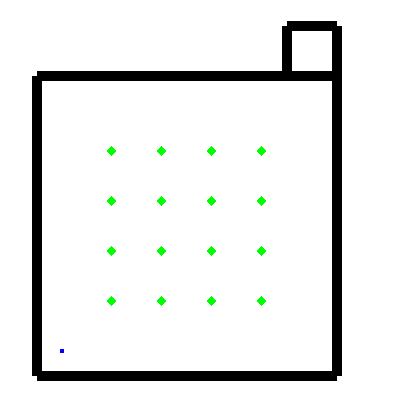
\includegraphics[scale=0.6]{figures/elderly_v3.png}
 \caption[認知症の場合の可視化]{認知症の場合の可視化 \label{elderly_v3}}
\end{center}
\end{figure}

\begin{figure}[htb]
\begin{center}
 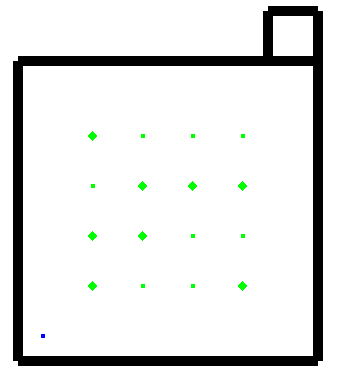
\includegraphics[scale=0.6]{figures/health_urinate.png}
 \caption[知的エージェントの模式図]{知的エージェントの模式図 \label{health_urinate}}
\end{center}
\end{figure}

\begin{figure}[htb]
\begin{center}
 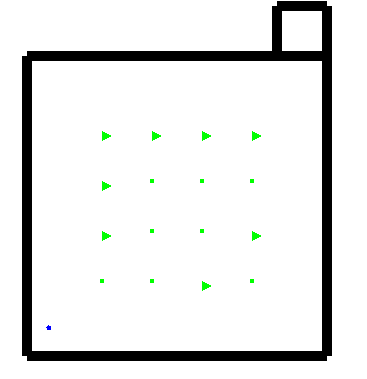
\includegraphics[scale=0.6]{figures/health_frequently_urinate_v1.png}
 \caption[知的エージェントの模式図]{知的エージェントの模式図 \label{health_frequently_urinate_v1}}
\end{center}
\end{figure}

\begin{figure}[htb]
\begin{center}
 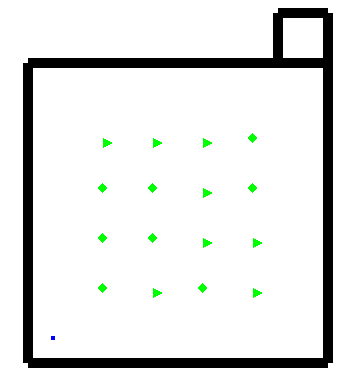
\includegraphics[scale=0.6]{figures/dementia_urinate_v1.png}
 \caption[知的エージェントの模式図]{知的エージェントの模式図 \label{dementia_urinate_v1}}
\end{center}
\end{figure}

\section{介護挙動の基本的な検証}

本シミュレータが現実を反映できているのかについて、簡単な検証を行った。
被介護者が、時系列で尿量が加算されて行き、その数値が健常者の場合は100mlを超えた時点で、頻尿の被介護者は〜を超えた時点で、認知症の被介護者は〜を超えた時点で、トイレに行きたいというアラートを発するように内部状態を設定した。その結果、健常者の場合は、2時間の間に1回トイレに行くという結果を得ることができた。これは実際のデータと比較しても整合性のある値となった。この結果を表\ref{被介護者ごとの排尿回数}に示す。なお、実験では16人の被介護者が存在するので実際は数値を16で割った数字が一人当たりの回数となっている。

\begin{table}[htb]
  \caption[被介護者ごとの排尿回数]{被介護者ごとの排尿回数}
  \label{model_explaination}
  \centering
  \begin{tabular}{r|c|c|c}
     & 健常者 & 頻尿 & 認知症 \\ \hline
    一回目 & 15 & 21 & 6 \\
    二回目 & 15 & 22 & 5 \\
    三回目 & 16 & 26 & 5 \\
    \end{tabular}
\end{table}

\section{評価指標}

CaseVの目的は、CaseIの分断のない場合からCaselVの完全分 断への過程 (経緯)を解析すること に あ る。1(遮断率0%)とIV(遮断率100% ) を 除 き 中 間値を4段階 (遮断率20・40・60・80%)とし、その経緯を 占有率、平均搬送距離、変更過程、変 更回数、負傷者の 収 容・未 収 容 か ら検 討する。個々の医療 施設としてだけで はなく、分 断 過 程 に お け る 同一地域内の医療 施設 群とし ても評価 する。さ ら に、負傷者が 互いに競合して影響し合 う関係 を分析する こ と で総食 的に評価す る。占有率が早期段階で満床にな らない揚合に は平均搬送距離は長距離となるが、平均搬送 距離を短距離とする に は遠距離の負傷者を収容しない で早期毅階で満床と な る こ と が 必 要である。つま り、全体のバラン ス について考察する こ と も 必 要 で あ る。
% 合計我慢時間と成功回数で評価する.
% 十分な量に達していないときに介護を行なった場合は過剰介護,待たせてしまった場合はお漏らし処理などの追加業務が発生する.

\section{結果および考察}

図8に,車 両発生率・歩行者発 生率を そ れ ぞ れ変 化さ せ た場 合の シ ミュレーション結 果(lo回の試行の平均値 )を不 す.比較のた め に,飽和 交通流率の琿論値も示す,車両発生率が500台/時 間以.ヒで歩 行者発 生率が20人/サ イク ル以 上の場 合には,シ ミュレーション結 果と埋論 値の差は12% 以内で あり,両者は よく一致しているといえる,一方,車 両発生率が200台/時 間以 下の場 合,お よ び歩行 者発生率が5入/ サイ クルのときには,シ ミュレーション結果 が 理論値よ りもか なり低 くなっている.こ 居しは,これ らの条件で は道路 が飽和していないた めに発生する相 違であると考えられる.
